\documentclass{beamer}

% THEME (Metropolis)
\usetheme[numbering=counter,progressbar=foot]{metropolis} % clean + progress bar
\usepackage{appendixnumberbeamer}

% FONTS (works with pdfLaTeX; for nicer system fonts, compile with XeLaTeX)
\usepackage[T1]{fontenc}
\usepackage[utf8]{inputenc}
\usepackage{lmodern}

% MATH / GRAPHICS
\usepackage{amsmath, amssymb}
\usepackage{graphicx}
\graphicspath{{figures/}}

% BIB (optional) — comment out if not needed
\usepackage[numbers]{natbib}
\usepackage{bibentry}

\usepackage{algorithm, algpseudocode}
\usepackage{float}

\usepackage{listings}
\usepackage{booktabs}        % for \toprule \midrule \bottomrule
\usepackage{xcolor} % for colors
\usepackage{adjustbox} % to scale only if needed
\definecolor{codebg}{RGB}{245,247,250}
\definecolor{codekw}{RGB}{0,90,160}
\definecolor{codecm}{RGB}{110,110,110}
\definecolor{codestr}{RGB}{160,60,60}
\definecolor{codenum}{RGB}{120,120,120}

\lstdefinestyle{nbody}{
  language=C,
  basicstyle=\footnotesize\ttfamily,    % smaller but still readable
  numbers=none,                          % ← no line numbers
  keywordstyle=\color{codekw}\bfseries,
  commentstyle=\color{codecm}\itshape,
  stringstyle=\color{codestr},
  backgroundcolor=\color{codebg},
  showstringspaces=false,
  tabsize=2,
  keepspaces=true,
  columns=fullflexible,
  breaklines=true, breakatwhitespace=true,
  aboveskip=2pt, belowskip=2pt,
  xleftmargin=0pt, framexleftmargin=0pt,
  frame=single, rulecolor=\color{black!10}, % subtle frame
}




% TITLE INFO
\titlegraphic{\includegraphics[width=0.35\textwidth]{black_unipv_logo_caption_right.png}}
\title{Scalability and Communication Overhead in Distributed N-Body Simulation using MPI on GCP}
\subtitle{\textit{Advanced Computer Architecture}}
\author{Claudio Guarrasi \\ \small{Department of Electrical, Computer and Biomedical Engineering} \\ \small{University of Pavia}}
\institute{}
\date{}
\begin{document}

% TITLE SLIDE
\maketitle

% AGENDA
\begin{frame}{Outline}
  \tableofcontents
\end{frame}

\section{Introduction}
\begin{frame}{Introduction}
\begin{itemize}
	\item N-Body problem is a well known problem in physics.
	\item Assumptions:
	\begin{itemize}
		\item Closed system containing $N$ point masses (bodies).
		\item No collisions.
		\item Gravitational interaction only $\Rightarrow \vec{F}_{i,j}=G\frac{m_{i} m_{j}}{\|\vec{r}_{i}-\vec{r}_{j}\|^3}(\vec{r}_{j}-\vec{r}_{i})$.
	\end{itemize}
	\item A closed-form solution does not exist\footnote{Douglas C. Heggie, \emph{The Classical Gravitational N-Body Problem}, arXiv:astro-ph/0503600 (2005).}.
	\item Numerical solution: solving equations of motion at each time step $k$.	
\end{itemize}
\end{frame}

\section{Physical Model}
\begin{frame}{Physical Model}
Underlying physics:
\begin{itemize}
	\item $\vec{F}_{i,j}=G\frac{m_{i} m_{j}}{\|\vec{r}_{i}-\vec{r}_{j}\|^3}(\vec{r}_{j}-\vec{r}_{i})$ (Gravitational universal law).
	\item $\Sigma\vec{F}_i = m_i\vec{a}_i$ (Newton's second law).
\end{itemize}
\begin{center}
	$\Downarrow$
\end{center}
\begin{itemize}
	\item $\vec{a}_i=\sum_{\substack{j=0 \\ j \neq i}}^{N-1}\left[G\frac{m_j}{\|\vec{r}_i-\vec{r}_j\|^3}(\vec{r}_j-\vec{r}_i)\right]$ (Acceleration of body $i$).
	\item $\vec{v}_i(t_k) = \vec{v}_i(t_{k-1}) + \int_{t_{k-1}}^{t_k} \vec{a}_i(\tau)\, d\tau \Rightarrow \vec{v}_{k+1}=\vec{v}_k+\vec{a}_k\Delta t$.
	\item $\vec{r}_i(t_k) = \vec{r}_i(t_{k-1}) + \int_{t_{k-1}}^{t_k} \vec{v}_i(\tau)\, d\tau \Rightarrow \vec{r}_{k+1}=\vec{r}_k+\vec{v}_k\Delta t$.
\end{itemize}
Direct method approach: expensive but more intuitive.
\end{frame}

\begin{frame}{Numerical Integration}
Not all numerical integration methods are good:
\begin{itemize}
	\item The exact velocity $v(t_{k+1})$ is: $v(t_k+\Delta t) = v(t_k) + a(t_k)\,\Delta t
+ \frac{\Delta t^2}{2} \frac{d^2 v}{dt^2}(\xi), \xi \in \left[ t_k,\, t_k+\Delta t \right]$
Step size $\Delta t$ weighs trade-off between accuracy and computational cost.
	\item Energy drift: $K_{TOT}(t_k) = \frac{1}{2} \sum_{i=0}^{N-1}m_iv_i^2(t_k)$
	\\Geometrical structure of the trajectories is not retained.
\end{itemize}
Symplectic methods prevent energy drift\footnote{R.~D.~Engle, “Monitoring energy drift with shadow Hamiltonians,” \emph{Journal of Computational Physics}, vol. 210, no. 2, pp. 371–384, 2005.} $\Rightarrow$ Semi-implicit Euler method: $\vec{r}_{k+1}=\vec{r}_k+\textcolor{red}{\vec{v}_{k+1}} \, \Delta t$
\end{frame}

\section{Serial Algorithm}
\begin{frame}{Serial Algorithm (Direct Method)}
Conceptual design of the serial algorithm
\begin{algorithm}[H]
\caption{Serial N-body algorithm (direct method)}
\label{alg:serial}
\begin{algorithmic}[1]
\State Initialize positions, velocities, and masses
\For{each time step}
    \State Compute accelerations (Algorithm~\ref{alg:inner_loop})
    \State Update velocities
    \State Update positions
\EndFor
\end{algorithmic}
\end{algorithm}
Space complexity:
$N \ \text{masses} + 3N \ \text{positions} + 3N \ \text{velocities} + 3N \ \text{accelerations} = 10N \ \text{real values} \Rightarrow O(N)$ 
\end{frame}

\begin{frame}{Serial Algorithm (Direct Method)}
\begin{algorithm}[H]
\caption{Inner loop: compute accelerations (direct method)}
\label{alg:inner_loop}
\begin{algorithmic}[1]
\Require Positions $\{\vec r_j\}_{j=0}^{N-1}$, masses $\{m_j\}_{j=0}^{N-1}$
\Ensure Accelerations $\{\vec a_i\}_{i=0}^{N-1}$
\For{$i \gets 0$ to $N-1$}
  \State $\vec a_i \gets (0,0,0)$
  \For{$j \gets 0$ to $N-1$}
    \If{$j \neq i$}
      \State $\vec a_i \gets \vec a_i + \text{effect of body}\, j \, \text{on body}\, i$
    \EndIf
  \EndFor
\EndFor
\Statex \textbf{Time complexity:} $O(N^2)$
\end{algorithmic}
\end{algorithm}
\end{frame}




\begin{frame}[fragile]{C Implementation}{}
Each major step of the Serial Algorithm mapped to a dedicated function.

\begin{lstlisting}[style=nbody]
void computePositions(int bodies, double dt){
  for (int i=0; i<bodies; ++i)
    positions[i] += dt * velocities[i]; }
\end{lstlisting}

\vspace{2mm}

\begin{lstlisting}[style=nbody]
void computeAccelerations(int bodies) {
    const double epsilon = 1e-5;
    for (int i = 0; i < bodies; i++) {
        accelerations[i] = 0.0;
        for (int j = 0; j < bodies; j++) {
            if (i != j) {
                double dist = positions[j] - positions[i] + epsilon;
                double invDistCubed = 1.0 / (dist * dist * dist);
                double scalar = GravConstant * masses[j] * invDistCubed;
                accelerations[i] += scalar * dist;            }
        }
    }
}
\end{lstlisting}

\end{frame}

\begin{frame}[fragile]{C Implementation: Profiling}
\centering

% --- Top row: two plots side by side ---
\begin{columns}[T,onlytextwidth]
  \column{0.5\textwidth}
  \centering
  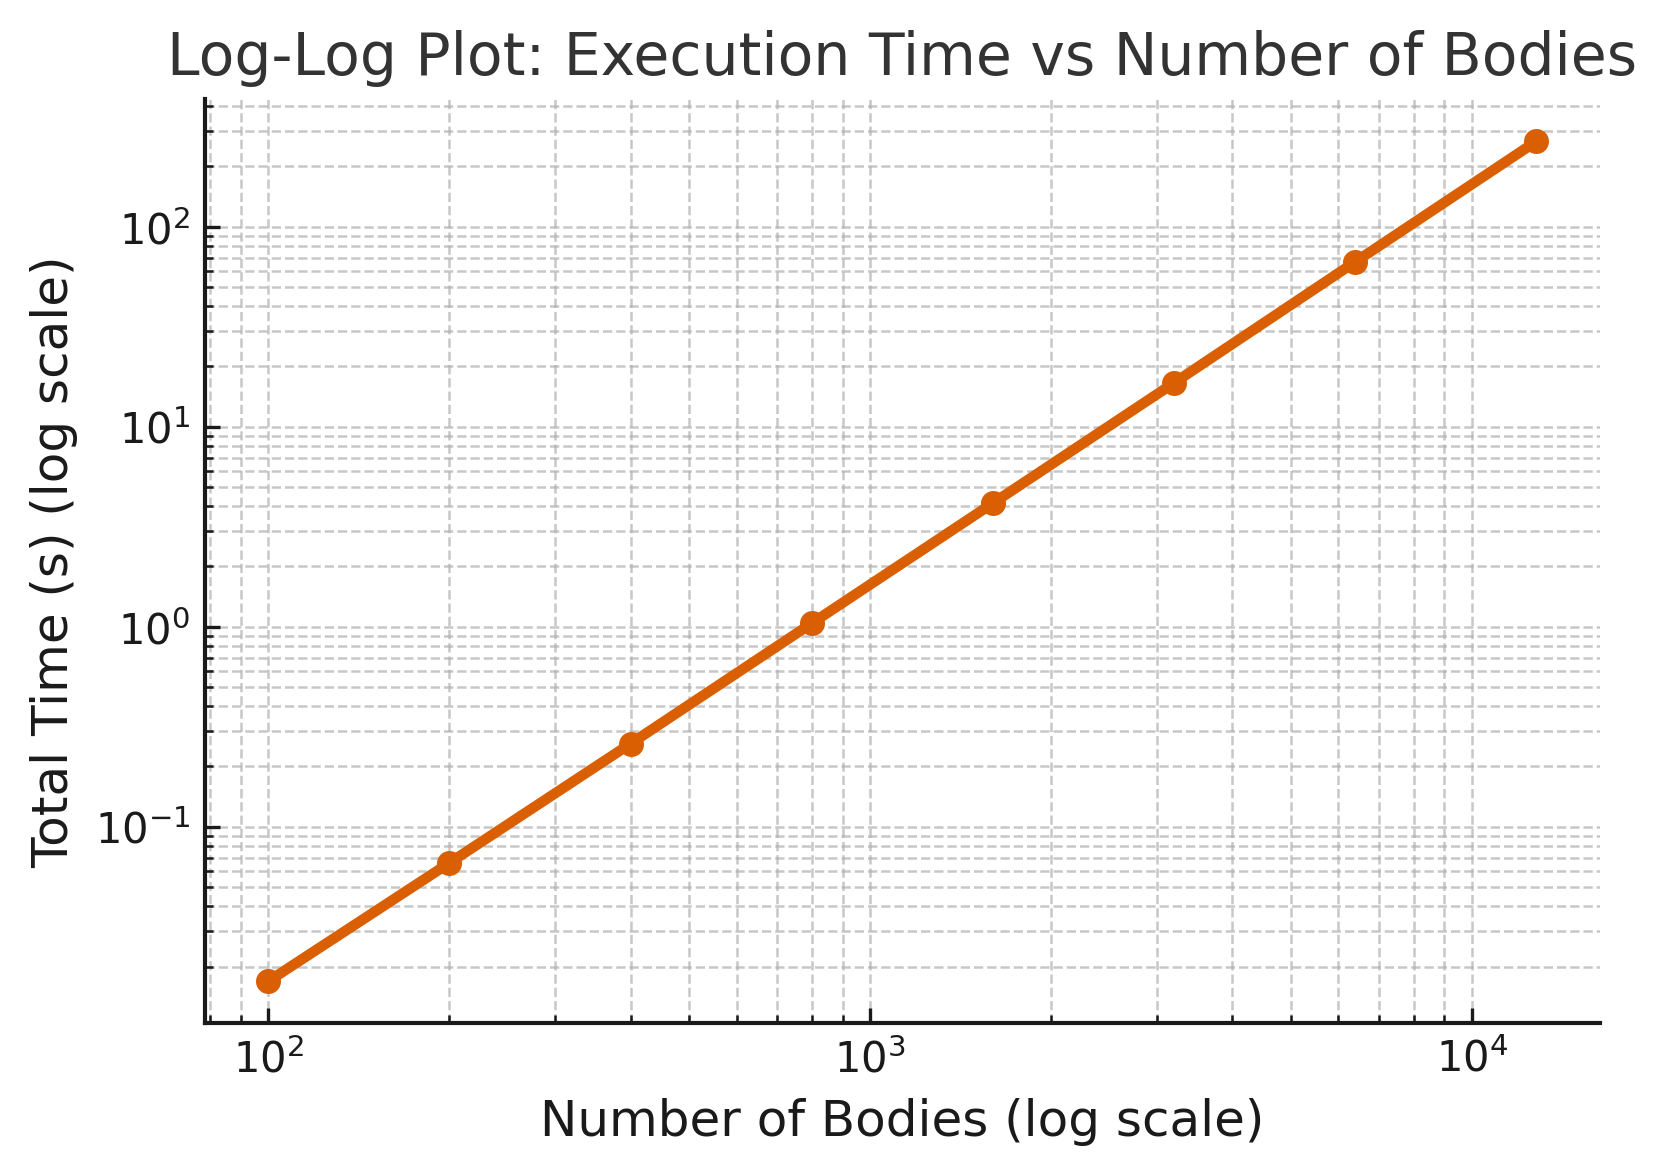
\includegraphics[width=0.6\linewidth]{logex_time_vs_logbodies.png}\\[1mm]
  {\footnotesize \textbf{Log–log:} execution time vs.\ bodies; power-law behavior.}

  \column{0.5\textwidth}
  \centering
  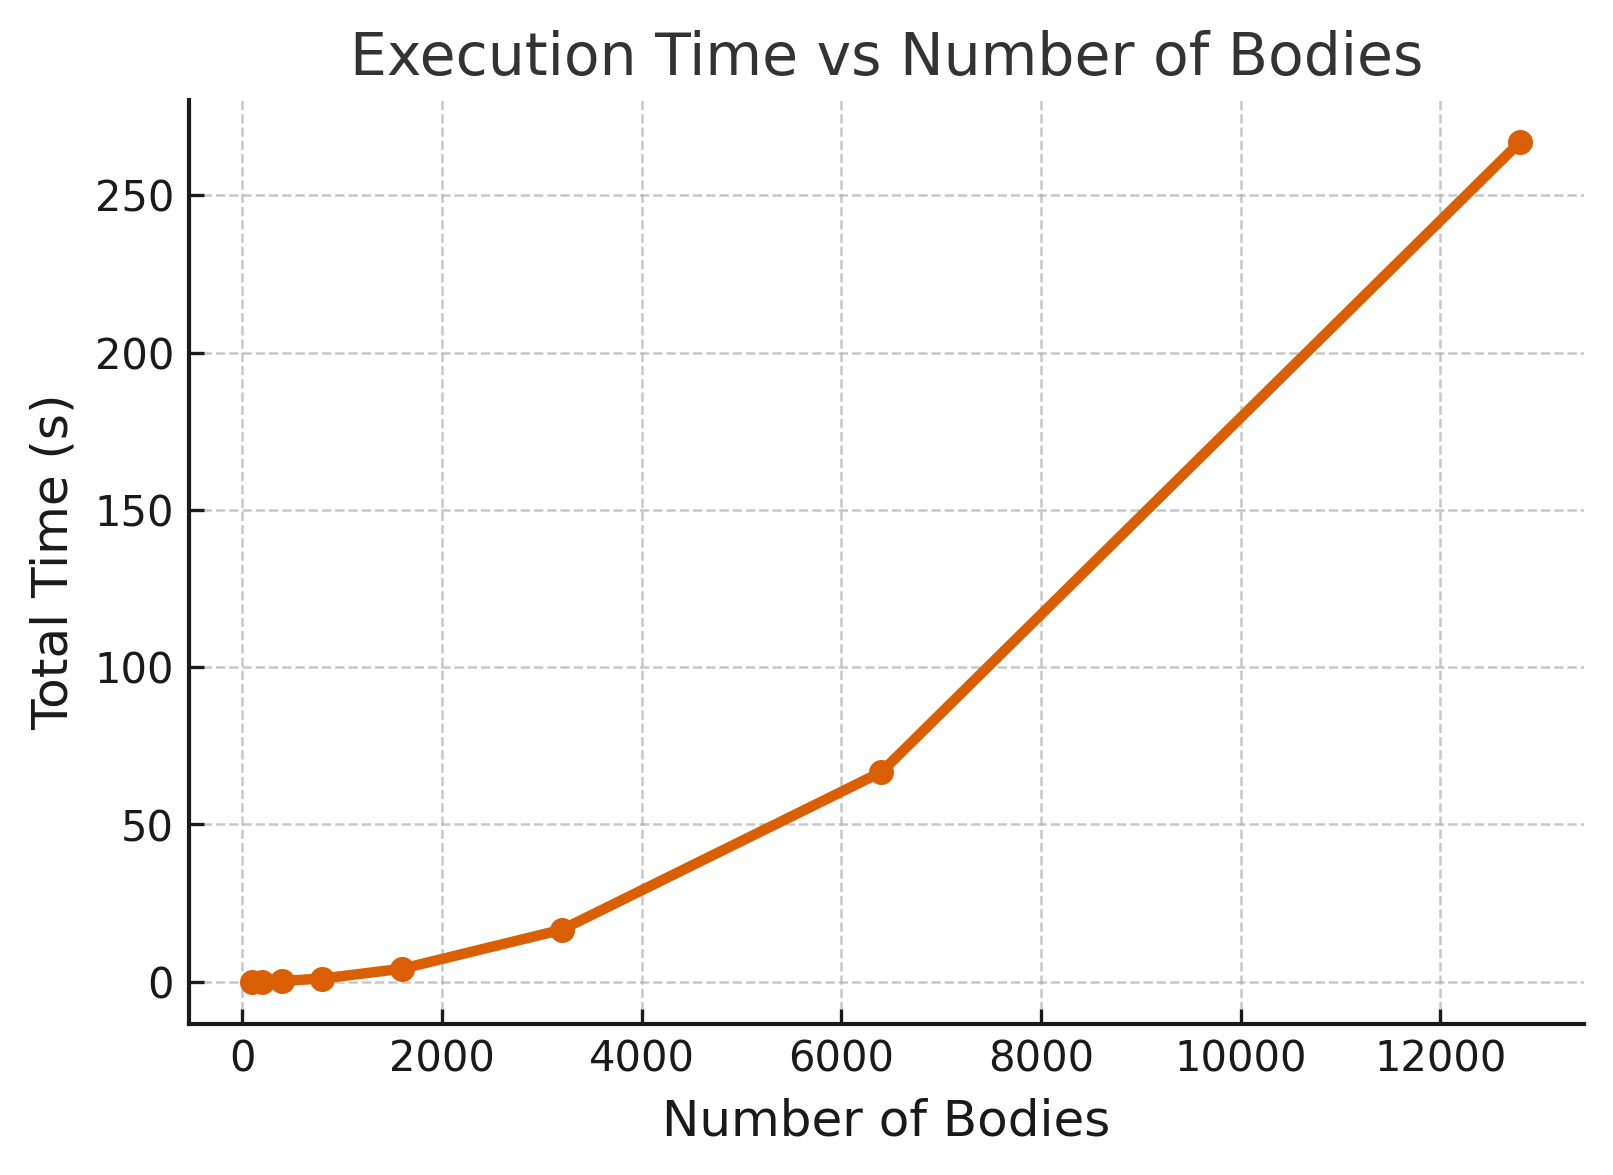
\includegraphics[width=0.6\linewidth]{ex_time_vs_bodies.png}\\[1mm]
  {\footnotesize \textbf{Linear:} execution time as a function of $N$.}
\end{columns}

\vspace{3mm}
\hrule % horizontal line separating plots from tables
\vspace{3mm}

% --- Bottom row: two verbatim blocks side by side with vertical line ---
\noindent
\begin{minipage}[t]{0.48\textwidth}
{\tiny
\begin{verbatim}
gprof Flat profile:

Each sample counts as 0.01 seconds.

  %   self  seconds  calls   name
 98.49 150.54   100   computeAccelerations
  1.49   2.28     -   _init
  0.01   0.02   100   computeVelocities
  0.01   0.01   101   logPositions
  0.00   0.00 60000   rand_uniform
  0.00   0.00   100   computePositions
  0.00   0.00   100   simulate
  0.00   0.00     1   initiateSystem
\end{verbatim}
}
\end{minipage}%
\hfill
\vrule width0.5pt % vertical separator
\hfill
\begin{minipage}[t]{0.48\textwidth}
{\tiny
\begin{verbatim}
 perf counter stats:

 Task-clock (ms)          268.400
 CPU Utilization          1.000 CPUs

 Cycles                   1.165e9 (4.341 GHz)
 Stalled-cycles-frontend  1.590e6
                          (0.14% frontend idle)

 Instructions             2.837e9 (2.43 IPC)
 Branches                 1.152e8
 Branch-misses            7.05e7
                         (0.06% of all branches)
\end{verbatim}
}
\end{minipage}

\end{frame}

\begin{frame}{C Implementation (A-priori Study of Available Parallelism)}
\begin{itemize}
  \item Amdahl's law (theoretical speedup):
\end{itemize}

\[
Speedup(N) = \frac{S+P}{S + \tfrac{P}{N}}
\]

\begin{itemize}
  \item For \texttt{computeAcceleration}: no loop-carried dependency. \\
        $\Rightarrow S=0,\; P=1$
  \item $\Rightarrow \; Speedup(N) = N$
  \item Ideal case: assumes communication among processes is instantaneous.
\end{itemize}
\end{frame}

\section{MPI Parallel Implementation}

\begin{frame}{MPI Parallel Implementation (Conceptual Design)}
\begin{algorithm}[H]
\caption{Parallel N-body (single-process view)}
\label{alg:parallel}
\begin{algorithmic}[1]
\State Initialize local positions, local velocities, and local masses
\State Send local positions and local masses
\State Wait for global positions and global masses
\For{each time step}
    \State Compute local accelerations (Algorithm~\ref{alg:parallel_inner_loop})
    \State Update local velocities
    \State Update local positions
    \State Send local positions
    \State Wait for global positions
\EndFor
\end{algorithmic}
\end{algorithm}
\end{frame}

\begin{frame}{MPI Parallel Implementation (Conceptual Design)}
\begin{algorithm}[H]
\caption{Parallel inner loop: compute local accelerations}
\label{alg:parallel_inner_loop}
\begin{algorithmic}[1]
\Require Global positions $\{\vec r_j\}_{j=0}^{N-1}$, global masses $\{m_j\}_{j=0}^{N-1}$
\Ensure Local accelerations $\{\vec a_i\}_{i=0}^{(N/P)-1}$
\For{each local body $i$}
  \State $\vec a_i \gets (0,0,0)$
  \For{$j \gets 0$ to $N-1$}
    \If{$j$ is not the same as global index of $i$}
      \State $\vec a_i \gets \vec a_i + \text{effect of body}\, j \, \text{on body}\, i$
    \EndIf
  \EndFor
\EndFor
\Statex \textbf{Time complexity (per process):} $O\!\left(\frac{N}{P} \cdot N\right) = O\!\left(\frac{N^2}{P}\right)$
\end{algorithmic}
\end{algorithm}
\end{frame}

\begin{frame}[fragile]{MPI Parallel Implementation (MPI\_Allgatherv)}
\texttt{MPI\_Allgatherv} is invoked as:
\begin{lstlisting}[style=nbody]
// each process contributes local_positions (b elements)
MPI_Allgatherv(
    local_positions, b, MPI_VECTOR,
    global_positions, recvcounts, displs,
    MPI_VECTOR, MPI_COMM_WORLD);
\end{lstlisting}

\begin{itemize}
  \item \textbf{Flexibility:} each process can contribute a different number of items 
        (via \texttt{recvcounts}).
  \item \textbf{Consistent ordering:} data placed in the same global order 
        (via \texttt{displs} offsets).
  \item \textbf{Blocking:} no process continues until all have finished exchanging data.
\end{itemize}
\end{frame}



\begin{frame}[fragile]{MPI Parallel Implementation (Initialization and Testing)}
\begin{itemize}
  \item Random initialization: seed depends on the \textbf{global index} of each body.  
        $\Rightarrow$ mirrors the serial version’s indexing scheme.
  \item Enables a \textbf{direct comparison} of serial vs.\ parallel output.
\end{itemize}

\vspace{2mm}

\textbf{Compute global start index (per process):}
\begin{lstlisting}[style=nbody]
unsigned int global_start_index(int r, int bodies, int rank) {
    if (rank < r) {
        return rank * (bodies + 1);
    } else {
        return r * (bodies + 1) + (rank - r) * bodies;
    }
}
\end{lstlisting}

\textbf{Seed formula:}
\begin{lstlisting}[style=nbody]
unsigned int seed = start_index + i;
\end{lstlisting}
\end{frame}

\section{Performance Evaluation on GCP}
\begin{frame}{Performance Evaluation on GCP}
\centering
\textbf{Experimental configurations of virtual instances}
\vspace{0.4cm}

\begin{tabular}{l l}
\toprule
\textbf{Setup} & \textbf{Description} \\
\midrule
Single fat & 1 × 16 vCPUs, 32 GB RAM, 1 region \\
Inter-regional fat & 2 × 8 vCPUs, 16 GB RAM, 2 regions \\
Intra-regional thin & 4 × 3 vCPUs, 3 GB RAM, 1 region \\
Inter-regional thin & 4 × 3 vCPUs, 3 GB RAM, 2 regions \\
Four-region thin & 4 × 3 vCPUs, 3 GB RAM, 4 regions \\
\bottomrule
\end{tabular}
\end{frame}


\begin{frame}{Performance Evaluation on GCP (Strong Scaling)}
\begin{itemize}
\item Theoretical strong scalability ($N_1=N_P$):
\end{itemize}
\[
Scalability(P) = \frac{t_{parallel}(1)}{t_{parallel}(P)} = \frac{N_1^2}{N_p^2}P = P
\]
\begin{itemize}
	\item Equivalent to study speedup since there is no inherently sequential part in the serial algorithm.
	\item Near-linear speedup up to 16 processes on one VM.
\end{itemize}
\vspace{0.5em}
\centering
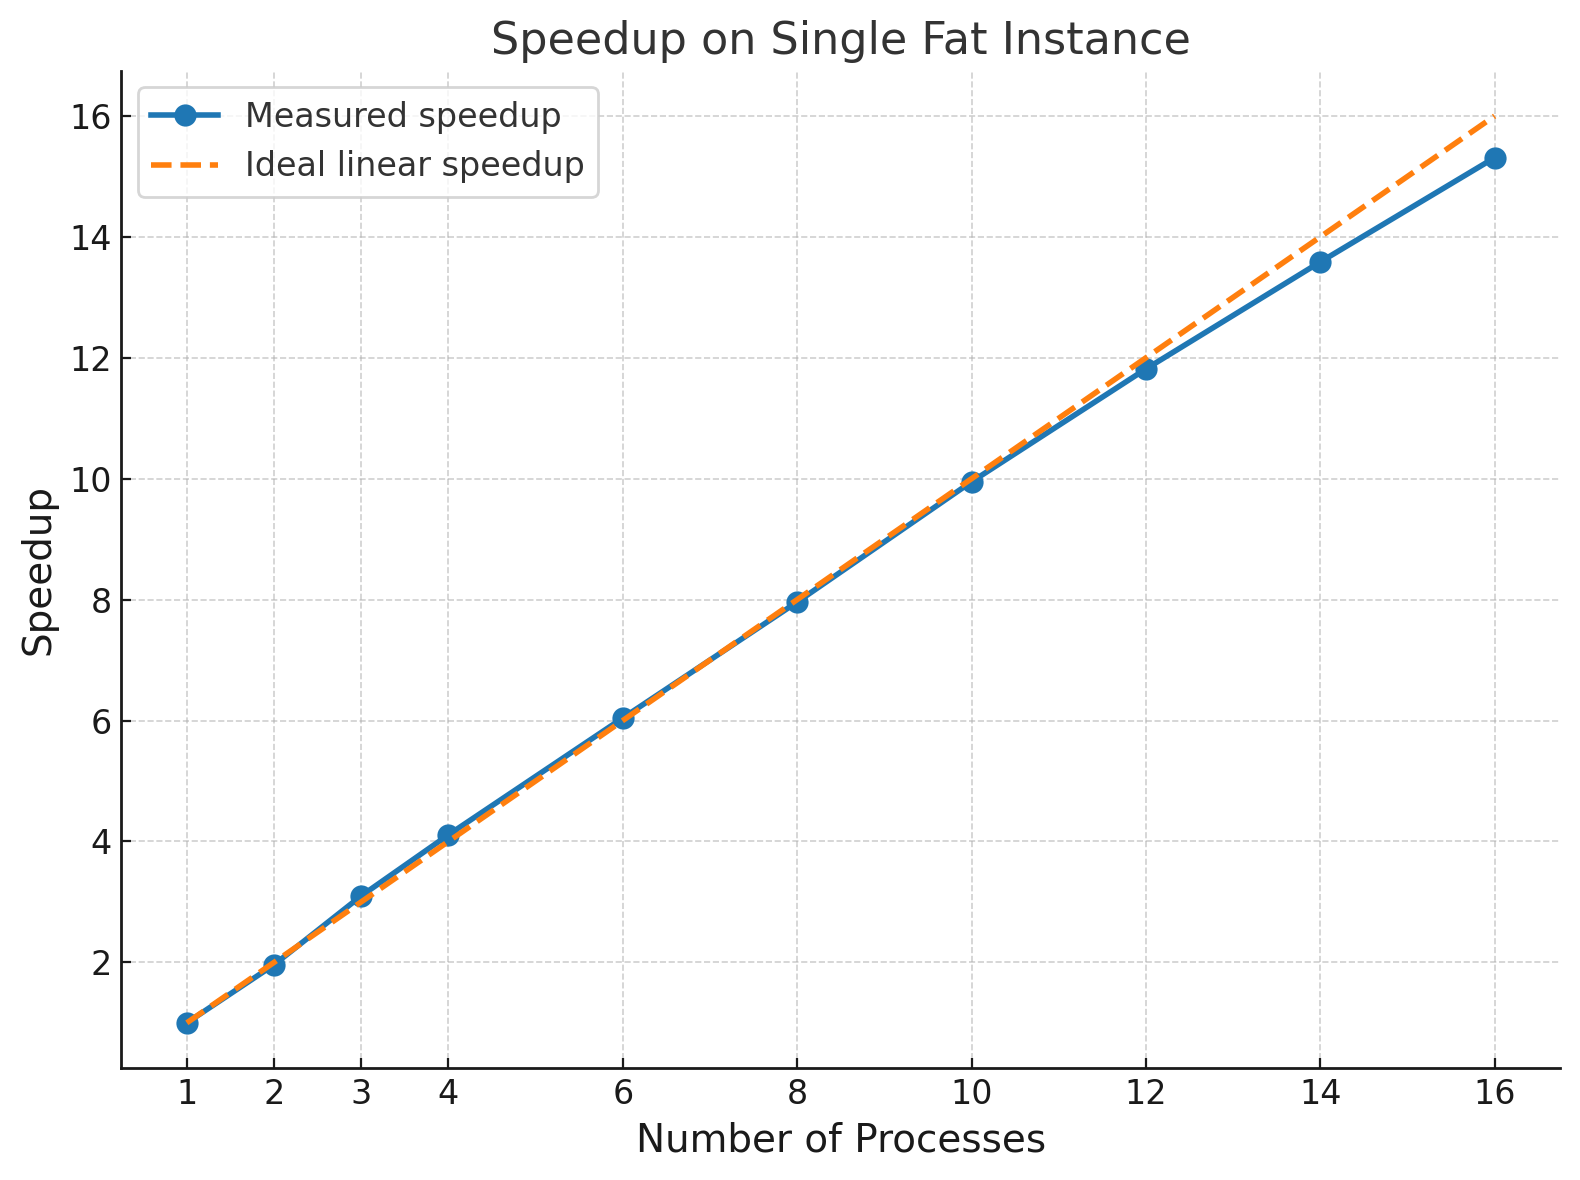
\includegraphics[width=0.5\linewidth]{parallel_strong_scaling_16_cores.png}
\end{frame}

\begin{frame}{Performance Evaluation on GCP (Strong Scaling)}
  \begin{itemize}
    \item Intra-regional clusters: negligible communication overhead.
    \item Inter-regional / multi-region: \texttt{MPI\_Allgatherv} becomes dominant.
  \end{itemize}
  \centering
  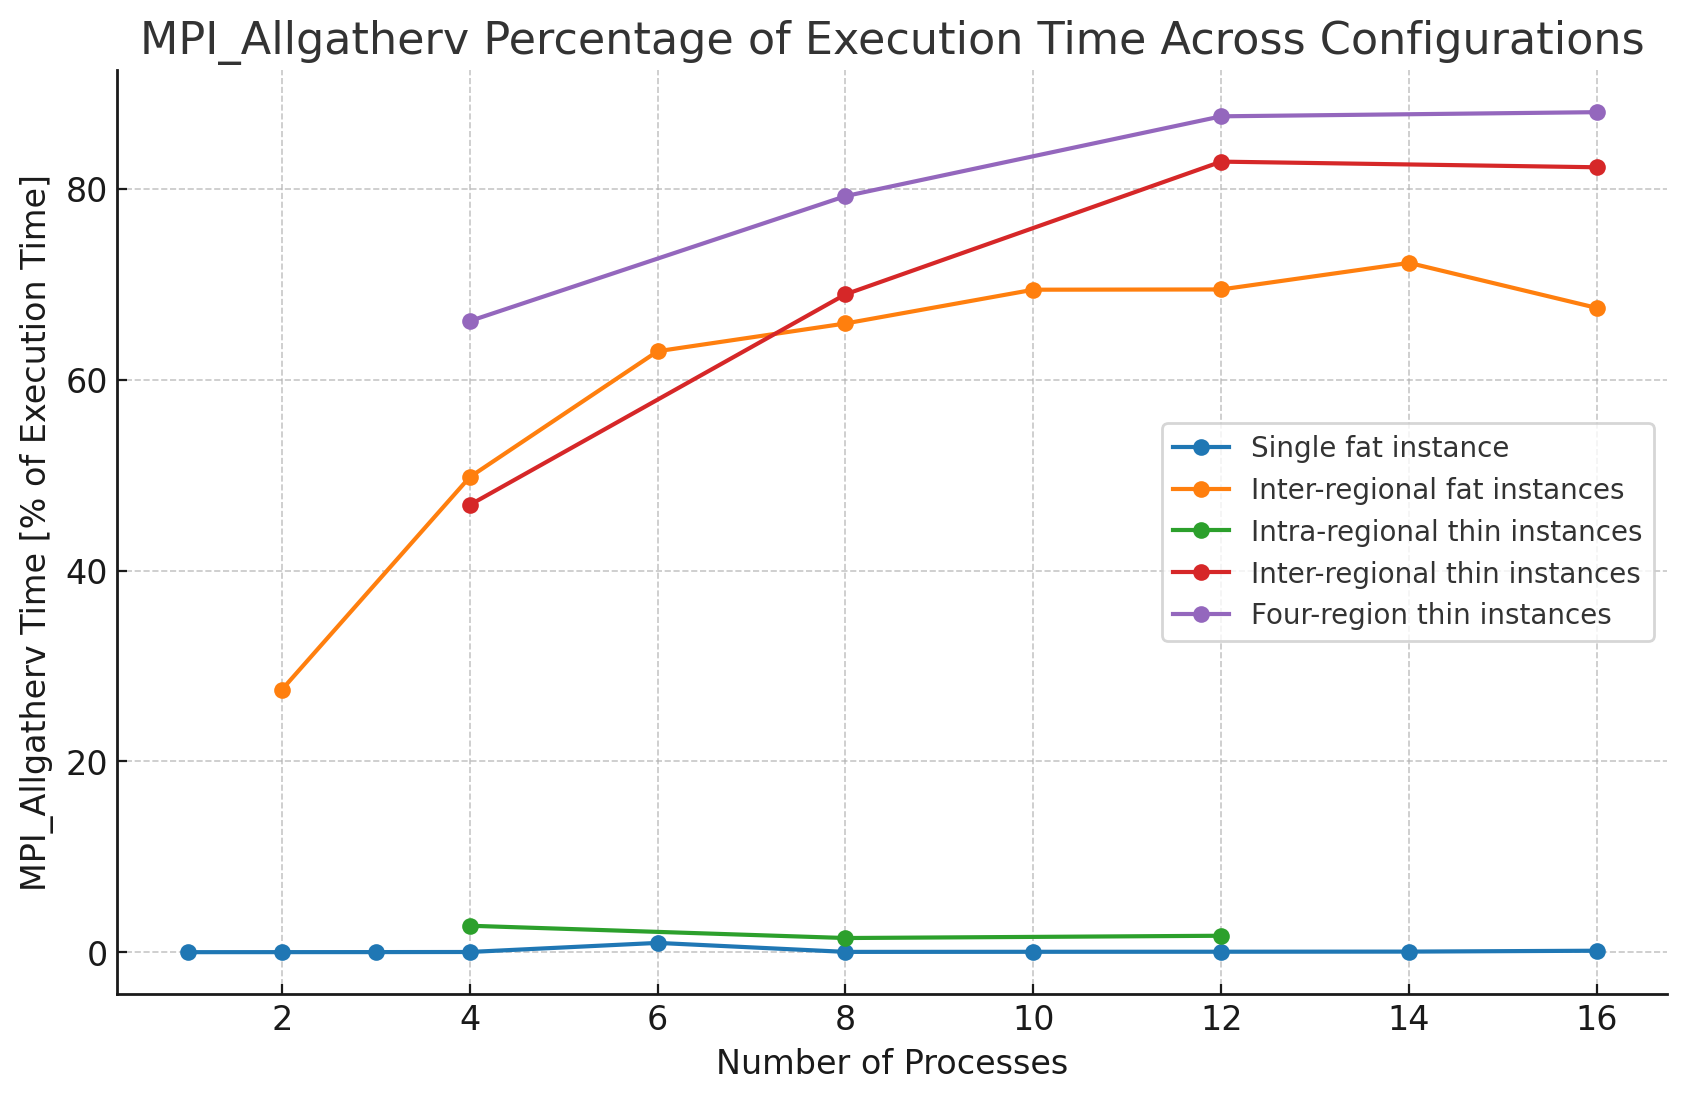
\includegraphics[width=0.85\linewidth]{communication_fraction_ex_time.png}
\end{frame}


\begin{frame}{Performance Evaluation on GCP (Weak Scaling)}
\begin{itemize}
	\item Theoretical weak scalability ($\tfrac{N_p}{P} = N_1$):
\end{itemize}
\[
Scalability(P) = \frac{t_{parallel}(1)}{t_{parallel}(P)} = \frac{N_1^2}{N_p^2}P = \frac{1}{P}
\]
\begin{itemize}
	\item The direct method inherently exhibits poor weak scalability, because each process must still loop over all $N$ bodies when computing accelerations.
\end{itemize}
  \centering
  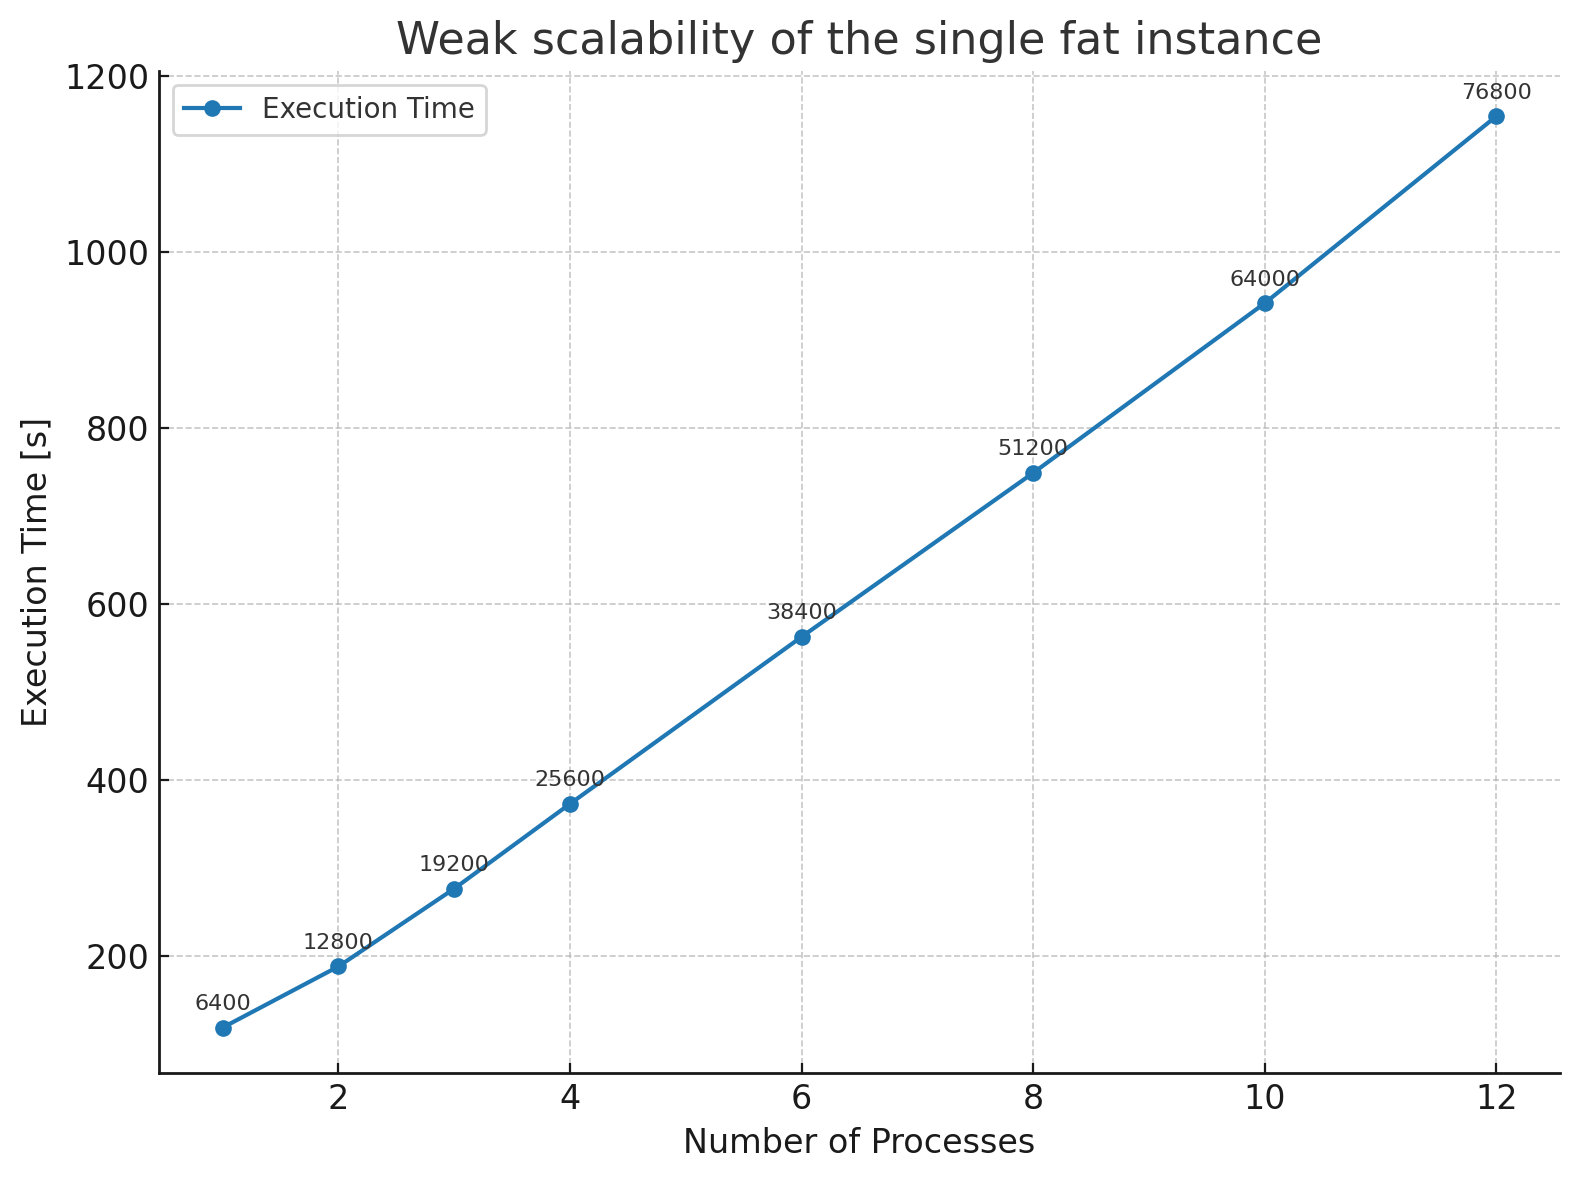
\includegraphics[width=0.47\linewidth]{parallel_weak_scalability.png}
\end{frame}

\begin{frame}{Conclusions}
  \begin{itemize}
    \item Strong scalability holds intra-node / intra-region.
    \item Inter-region latency breaks scalability (blocking collective).
    \item Direct $O(N^2)$ method limits weak scalability.
    \item Future work: hierarchical/approximate methods (e.g., Barnes--Hut).
  \end{itemize}
\end{frame}















%%%%%%%%%%%%%%%%%%%%%%%%%%%%%%%%%%%%%%%%%%%%%%%%%5
\begin{frame}{N-Body Problem}
N-Body Problem is a well known problem in physics. \\
Applications include:
\begin{itemize}
    \item Modeling gravitational interactions in galaxies.
    \item Simulating charged particle dynamics.
    \item Describing particles in visual effects (smoke, dust, and so on).
    \item $\cdots$
\end{itemize}
\end{frame}






\begin{frame}{N-Body Problem (Model)}
Assumptions:
\begin{itemize}
	\item Closed system containing $N$ point masses.
	\item No collisions.
	\item Gravitational interaction only $\Rightarrow \vec{F}_{i,j}=G\frac{m_{i} m_{j}}{\|\vec{r}_{i}-\vec{r}_{j}\|^3}(\vec{r}_{j}-\vec{r}_{i})$.
\end{itemize}
Enough for computing the trajectories of celestial bodies since their masses are very large with respect to the distances.


\end{frame}

\begin{frame}{N-Body Problem (Model)}
Dynamics of the model
\begin{enumerate}
	\item $N$ point masses (bodies) interacts with one another.
	\item Each body $i$ it is subject to a resulting force $\Sigma F$ obtained by summing all the gravitational forces exerted by the others $N-1$ bodies in the system.
	\item Given the mechanics fundamental law $\Sigma\vec{F}_i = m_i\vec{a}_i$, the acceleration $\vec{a}_i$ of body $i$ can be computed as:
	\begin{center}
	$\vec{a}_i=\sum_{\substack{j=0 \\ j \neq i}}^{N-1}\left[G\frac{m_j}{\|\vec{r}_i-\vec{r}_j\|^3}(\vec{r}_j-\vec{r}_i)\right]$
	\end{center}  
\end{enumerate}
\end{frame}

\begin{frame}{N-Body Problem (Model)}
Integrating from $\vec{a}_i$ we obtain: 
\begin{itemize}
	\item $\vec{v}_i(t_k) = \vec{v}_i(t_{k-1}) + \int_{t_{k-1}}^{t_k} \vec{a}_i(\tau)\, d\tau$.
	\item $\vec{r}_i(t_k) = \vec{r}_i(t_{k-1}) + \int_{t_{k-1}}^{t_k} \vec{v}_i(\tau)\, d\tau$.  
\end{itemize}
where $t_{k-1}$ is the time instant defining the initial condition for the current time step.
\\
Why do we not put just $\vec{v}_i(t_{k-1}) = \vec{v}_i(0)$ and $\vec{r}_i(t_{k-1}) = \vec{r}_i(0)$?
\end{frame}

\begin{frame}{N-Body Problem (Model)}
\begin{itemize}
	\item For \( N > 2 \), the N-body problem does not admit a general closed-form solution.%: it is not possible to determine the complete trajectories of all bodies analytically from the initial conditions alone.
	\item To compute the position of one particular mass at time $k$ it is necessary to compute the positions $\vec r$ of all the $N$ bodies at each time step $t \leq k$. $\Rightarrow$ Numerical solution% This is required because, as shown in \eqref{eq:acceleration}, the acceleration at time $k$ depends on the positions of all the bodies at that time.
\end{itemize}
Just from this consideration we can already anticipate the high computational cost.
\end{frame}


\begin{frame}{Scope of the work}
What it has been done:
\begin{enumerate}
\item to analyze a possible serial algorithm for solving the N-body problem;
\item to perform an \emph{a priori} study of the available parallelism using Amdahl's Law;
\item to develop a parallel implementation using the Message Passing Interface (MPI);
\item to evaluate performance and scalability through experiments conducted on Google Cloud Platform (GCP).
\end{enumerate}
\end{frame}

\begin{frame}{Serial Algorithm}
How can we numerically solve the N-Body problem?  
Main approaches:
\begin{itemize}
    \item \textbf{Direct method:} each particle interacts with all others. Accurate but $O(N^2)$ costly.%it most closely reflects the conceptual formulation of the problem. It is more expensive.
    \item \textbf{Barnes–Hut:} hierarchical tree (quad/octree); distant bodies approximated by center of mass. $O(N \log N)$.%Barnes-Hut method, organizes bodies in a tree structure, each leaf contains a single body or a small group of bodies. %(approximation).
    \item \textbf{Particle–Mesh:} space discretized into a grid; mass density $\rightarrow$ potential (FFT); forces interpolated back to particles. $O(N + M \log M)$. %the space is divided into grids (meshes), gravitational potential is computed based on the mass density of the bodies in a grid. ANd then Forces computed on grid and then interpolated back to particles.
    \item $\cdots$
\end{itemize}
\end{frame}

\begin{frame}{Serial Algorithm (Direct Method)}
Transitioning to discrete-time domain:
\begin{itemize}
	\item $\vec{v}_i(t_k) = \vec{v}_i(t_{k-1}) + \int_{t_{k-1}}^{t_k} \vec{a}_i(\tau)\, d\tau$.
	\item $\vec{r}_i(t_k) = \vec{r}_i(t_{k-1}) + \int_{t_{k-1}}^{t_k} \vec{v}_i(\tau)\, d\tau$.
\end{itemize}
\begin{center}
$\Downarrow$
\end{center}
\begin{itemize}
	\item $\vec{v}_{k+1}=\vec{v}_k+\vec{a}_k\Delta t$.
	\item $\vec{r}_{k+1}=\vec{r}_k+{v}_k\Delta t$.
\end{itemize}
Please note that $\Delta t$ is the step size between two consecutive time instants.
Incidentally, we expressed position and velocity using the explicit Euler method.

Is it the right numerical integration method? 
\end{frame}

\begin{frame}{Numerical Integration}
The exact velocity $v(t_{k+1})$ at time step $k+1$ using the Taylor expansion with Lagrange remainder is:
$
\begin{aligned}
v(t_k+\Delta t) = v(t_k) + a(&t_k)\,\Delta t
+ \frac{\Delta t^2}{2} \frac{d^2 v}{dt^2}(\xi),
&\quad \xi \in \left[ t_k,\, t_k+\Delta t \right]
\end{aligned}
$
\begin{itemize}
	\item Numerical integration method produce approximations.
	\item Step size $\Delta t$ weighs trade-off between accuracy and computational cost. %DA RIVEDERE
\end{itemize}
\end{frame}

\begin{frame}{Numerical Integration (Energy Drift)}
The numerical error accumulates $\Rightarrow$ Energy Drift \\[2ex]
\begin{center}
$K_{TOT}(k) = \frac{1}{2} \sum_{i=0}^{N-1}m_iv_i^2(k)$
\end{center}
If the total energy $K_{TOT}$ keeps increasing the simulated system %assumed to be closed
may turn "unstable", i.e., it is not retained the geometrical structure of the trajectories.
\end{frame}

\begin{frame}{Numerical Integration (Symplectic Methods)}
It can be proven that a \emph{symplectic} numerical methods allow to bound the energy oscillations around the true value, avoiding energy drift.  %cita con nota a pie di pagina
\\[2ex]
Semi-implicit Euler method has been chosen:
\begin{itemize}
	\item $\vec{v}_{k+1}=\vec{v}_k+\vec{a}_k\Delta t $
	\item $\vec{r}_{k+1}=\vec{r}_k+\textcolor{red}{\vec{v}_{k+1}} \, \Delta t$
\end{itemize}
%The only difference is that to compute the position at time step $k+1$ we use the updated velocity %$v_{k+1}$ and not the velocity at the previous time step $k$
\end{frame}
 \begin{frame}{Why no closed-form solution for N-Body?}
\begin{itemize}
    \item Newton’s equations for $N$ bodies $\Rightarrow$ system of $6N$ coupled ODEs:
    \[
        m_i \ddot{\mathbf{r}}_i = G \sum_{j \neq i} \frac{m_i m_j}{|\mathbf{r}_i - \mathbf{r}_j|^3} (\mathbf{r}_j - \mathbf{r}_i)
    \]
    \item For $N=2$: reduces to a central force problem $\Rightarrow$ Kepler’s laws, closed-form ellipses.  
    \item For $N \geq 3$:  
        \begin{itemize}
            \item Equations are \textbf{non-linear} and \textbf{mutually coupled}.  
            \item No general change of coordinates decouples the system.  
            \item Proven chaotic dynamics (Poincaré, 1890): no closed-form integrals beyond energy, momentum, angular momentum.  
        \end{itemize}
    \item $\Rightarrow$ Only special symmetric cases (e.g. restricted 3-body, Lagrange points) have analytic solutions.  
    \item In general, we must resort to \textbf{numerical integration}.  
\end{itemize}
\end{frame}



%%%%%%%%%%%%%%%%%%%%%%%%%%%%%%%%%%%%%%%





\section{Problem \& Model}
\begin{frame}{N-Body Problem (Direct Method)}
  \begin{itemize}
    \item $N$ point masses, gravitational interaction only.
    \item Direct method: compute all pairwise forces $\Rightarrow O(N^2)$.
    \item Parallelization goal: distribute bodies and keep a global view of positions.
  \end{itemize}
  \vspace{0.5em}
  \textbf{Key equation:}
  \[
    \vec{a}_i=\sum_{\substack{j=0 \\ j \neq i}}^{N-1}
    \left[G\frac{m_j}{\|\vec{r}_i-\vec{r}_j\|^3}(\vec{r}_j-\vec{r}_i)\right]
  \]
\end{frame}

\section{Method}
\begin{frame}{MPI Parallelization at a Glance}
  \begin{columns}[T,totalwidth=\textwidth]
    \column{0.55\textwidth}
    \begin{itemize}
      \item Bodies split across $P$ processes ($\approx N/P$ each).
      \item Each step:
      \begin{enumerate}
        \item Allgather positions (and once masses).
        \item Compute local accelerations.
        \item Update velocities/positions.
      \end{enumerate}
      \item Uses \texttt{MPI\_Allgatherv} (blocking, collective).
    \end{itemize}
    \column{0.42\textwidth}
    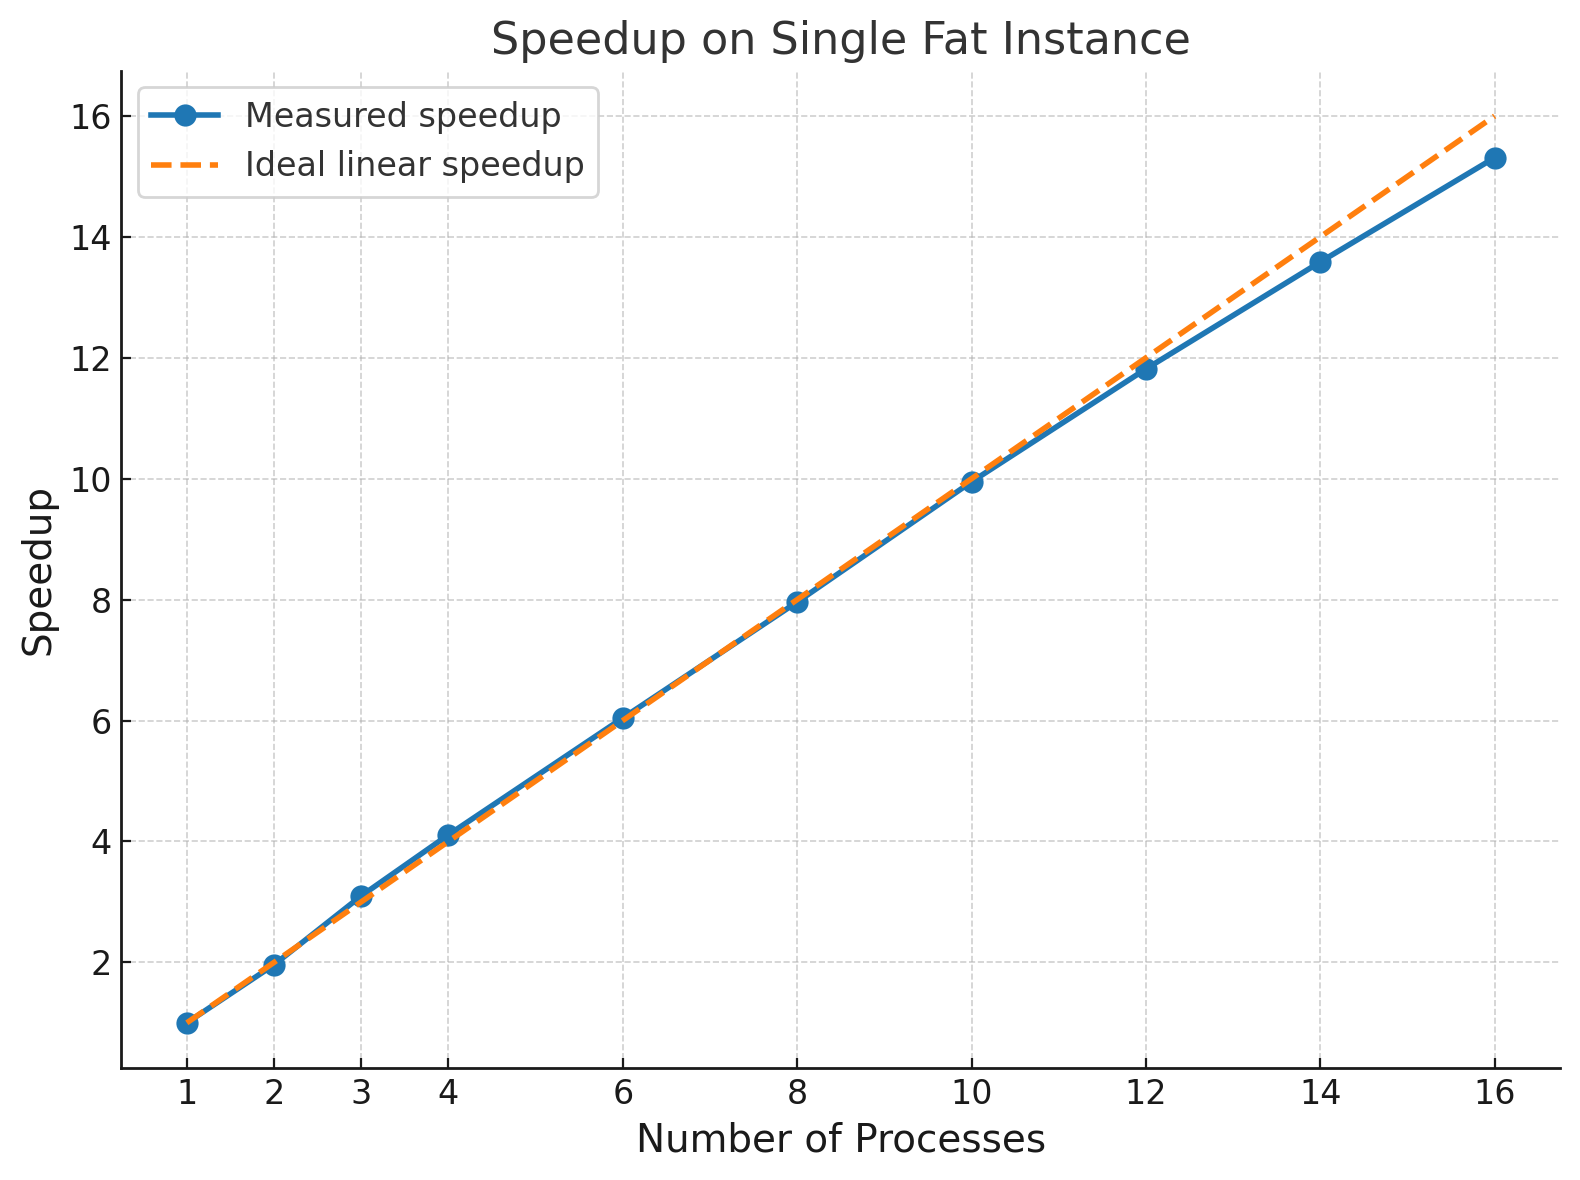
\includegraphics[width=\linewidth]{parallel_strong_scaling_16_cores.png}
    \vspace{0.3em}
    \scriptsize Example plot placeholder
  \end{columns}
\end{frame}

\section{Results}
\begin{frame}{Strong Scalability (Single Fat Instance)}
  \begin{itemize}
    \item Near-linear speedup up to 16 processes on one VM.
    \item Communication time is negligible intra-node.
  \end{itemize}
  \vspace{0.5em}
  \centering
  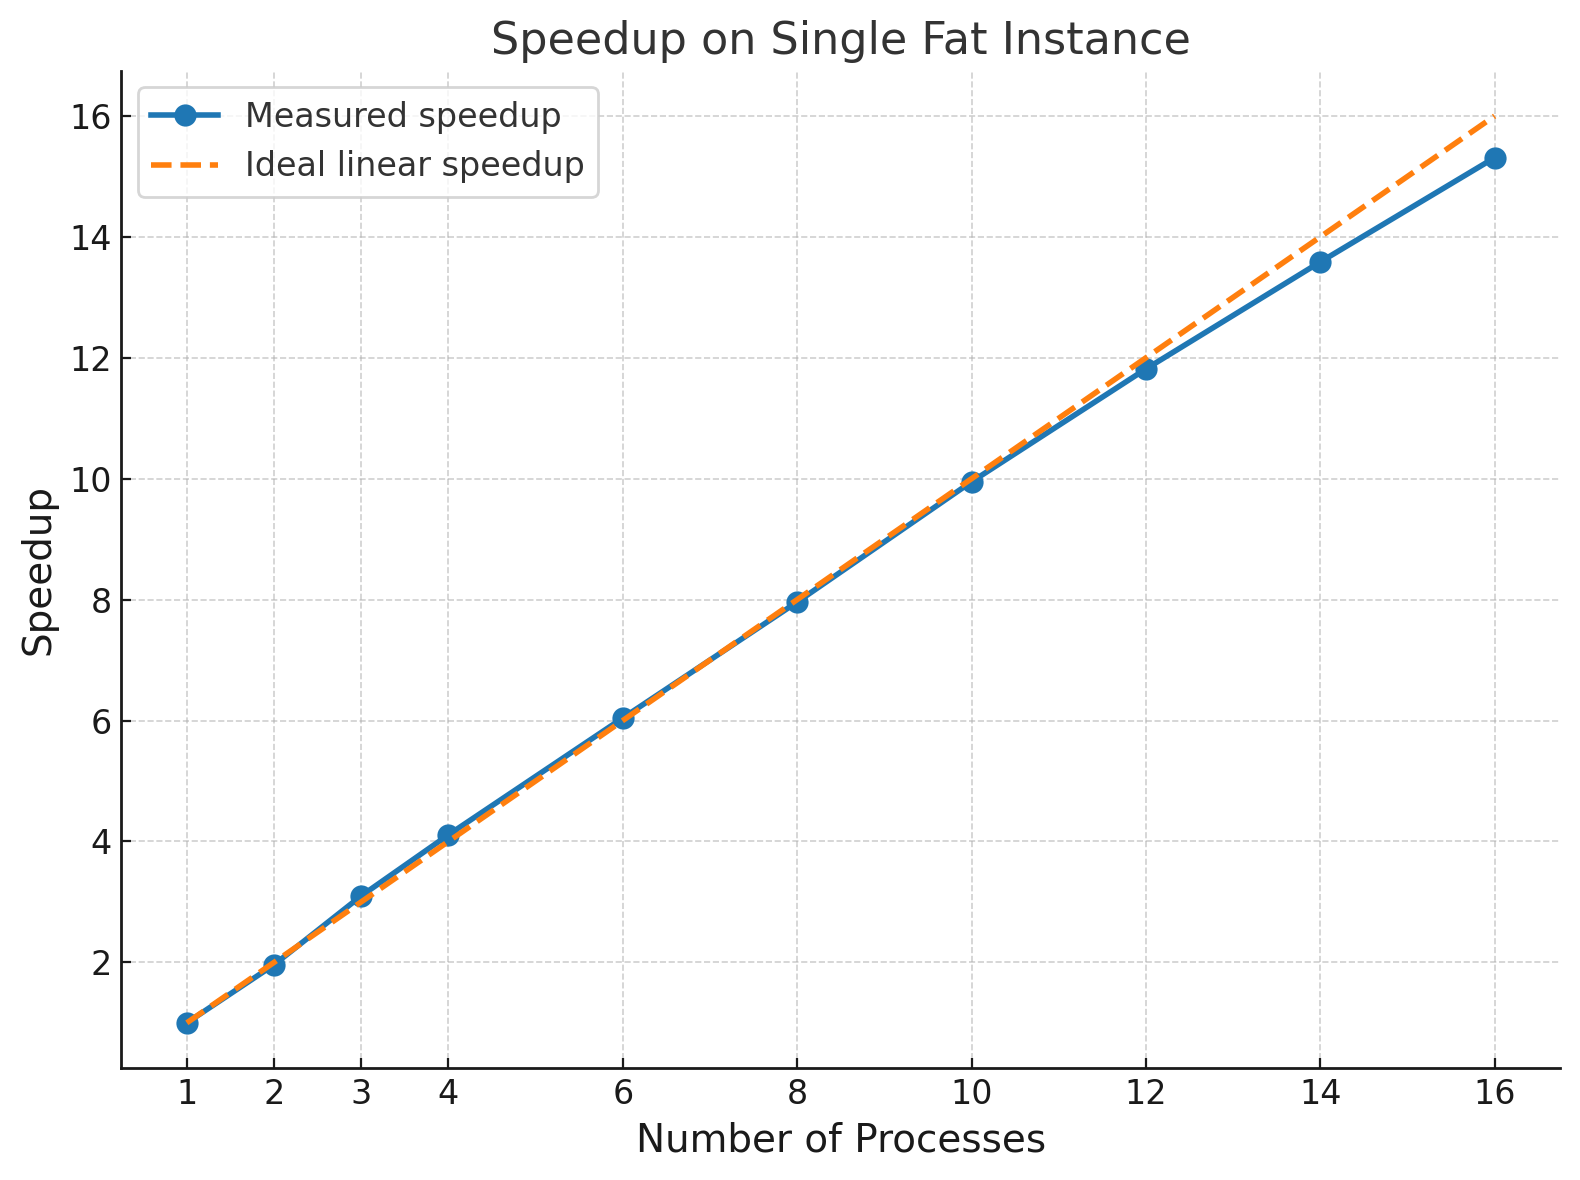
\includegraphics[width=0.8\linewidth]{parallel_strong_scaling_16_cores.png}
\end{frame}

\begin{frame}{Communication Overhead Across Configurations}
  \begin{itemize}
    \item Intra-regional clusters: modest overhead.
    \item Inter-regional / multi-region: \texttt{MPI\_Allgatherv} becomes dominant.
  \end{itemize}
  \centering
  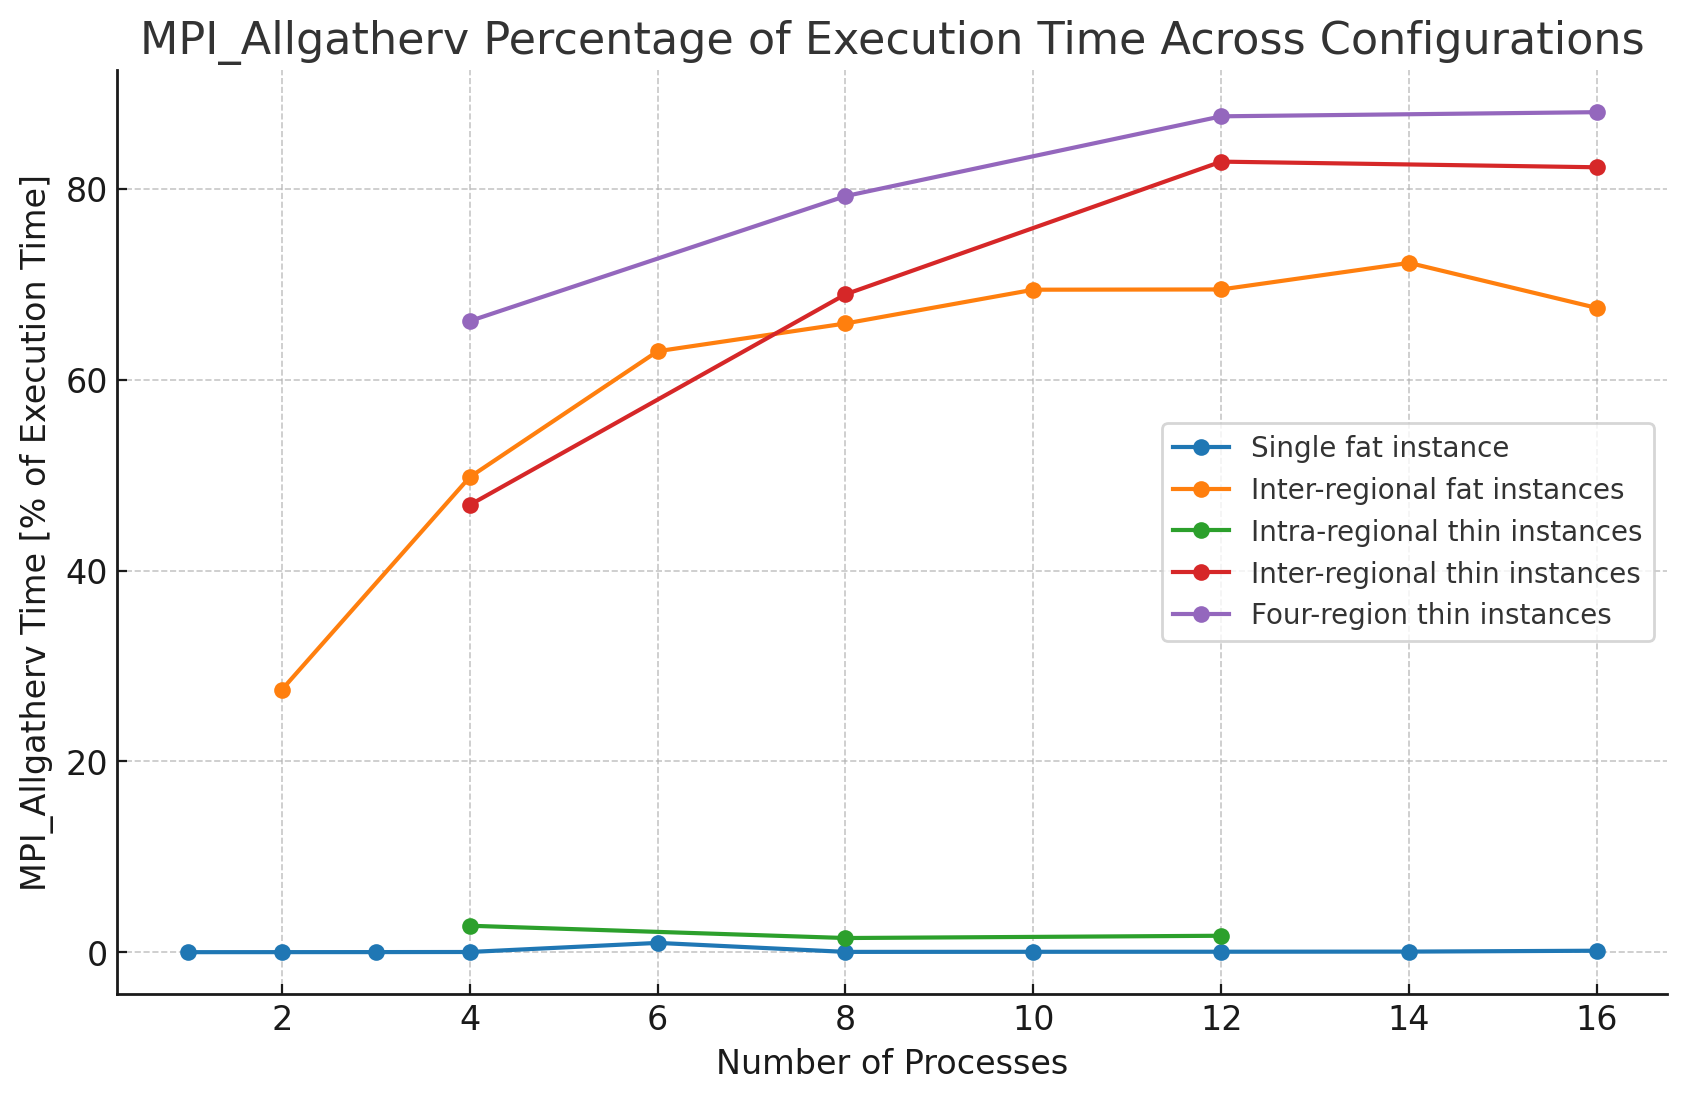
\includegraphics[width=0.85\linewidth]{communication_fraction_ex_time.png}
\end{frame}

\begin{frame}{Weak Scalability (Direct Method)}
  \begin{itemize}
    \item With $N \propto P$, per-process data is constant, but
    \item Per-process \emph{computational} work $\sim O(N^2/P)\propto P$.
    \item Runtime grows with $P$ (poor weak scalability).
  \end{itemize}
  \centering
  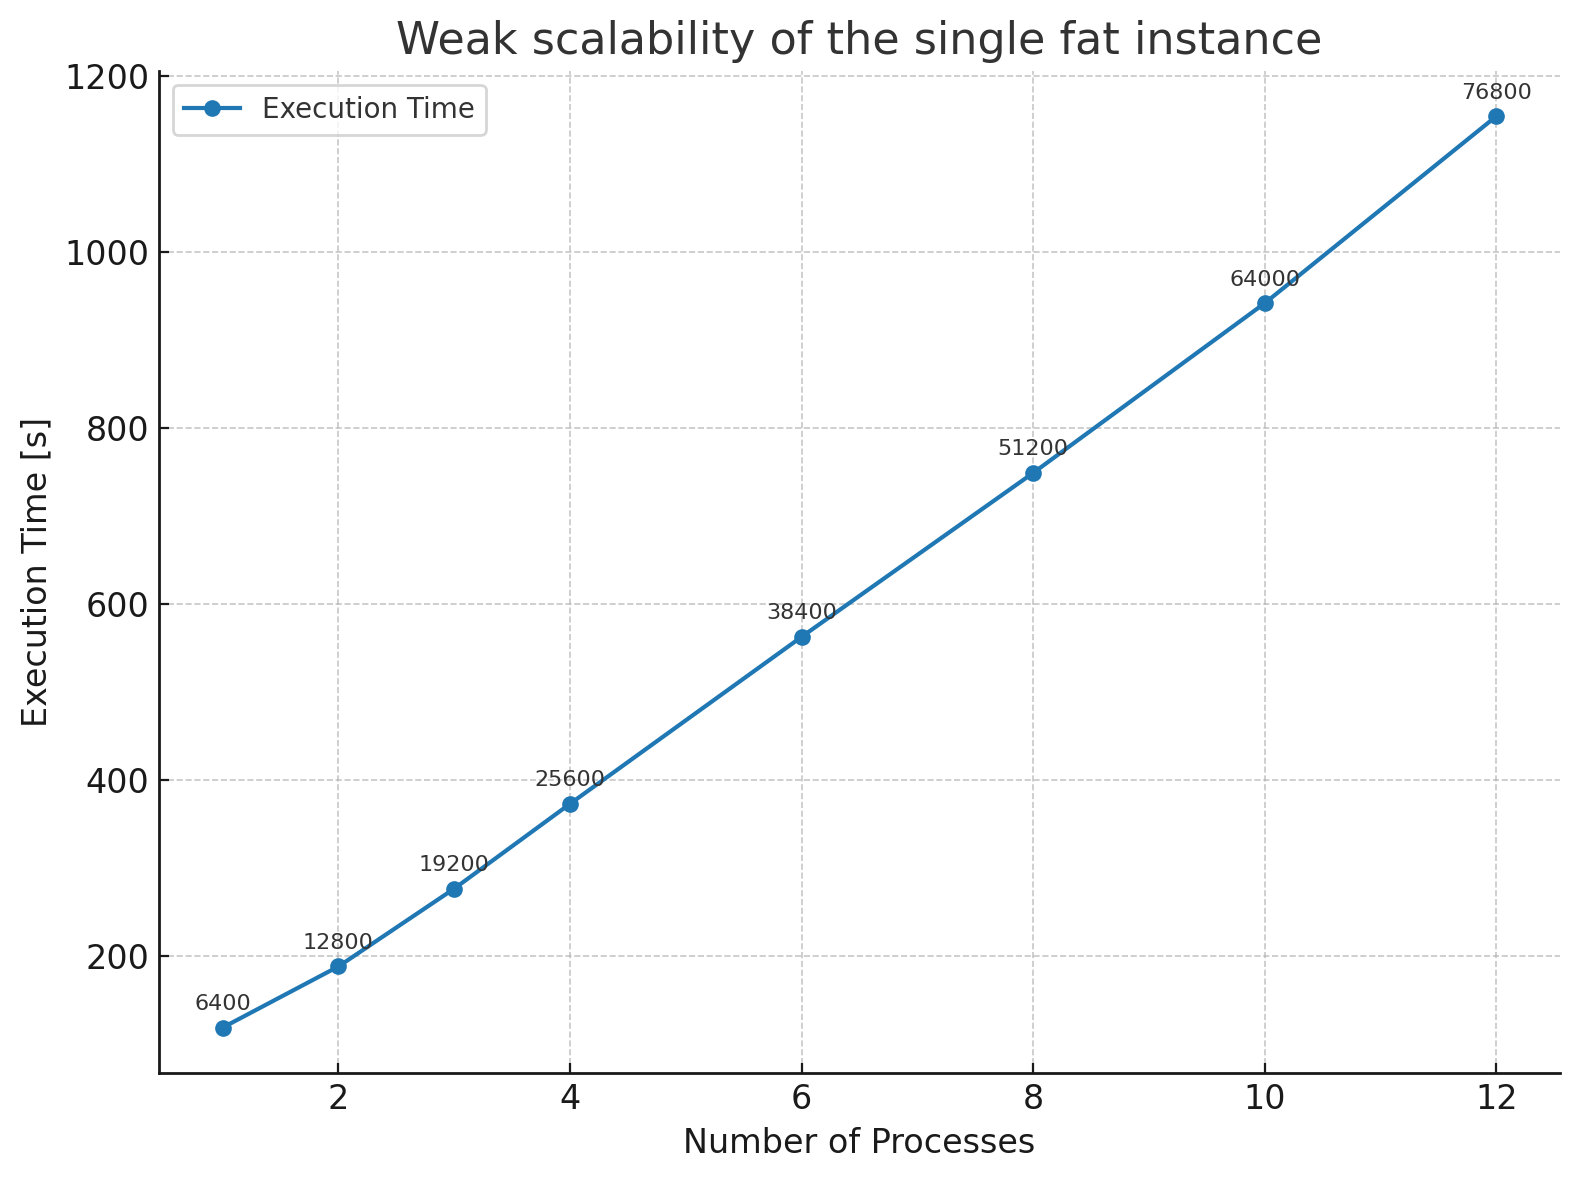
\includegraphics[width=0.8\linewidth]{parallel_weak_scalability.png}
\end{frame}

\section{Takeaways}
\begin{frame}{Conclusions}
  \begin{itemize}
    \item Strong scalability holds intra-node / intra-region.
    \item Inter-region latency breaks scalability (blocking collective).
    \item Direct $O(N^2)$ method limits weak scalability.
    \item Future work: hierarchical/approximate methods (e.g., Barnes--Hut).
  \end{itemize}
\end{frame}

\begin{frame}[standout]
  Questions?
\end{frame}

% OPTIONAL: References slide
% \begin{frame}[allowframebreaks]{References}
%   \small
%   \bibliographystyle{unsrtnat}
%   \bibliography{references}
% \end{frame}

\end{document}

